\documentclass[%
    school=etsisi,%
    degree=61TI,%
]{upm-report}

\title{Práctica 1: Diseño de un centro de datos bare metal}
\author{Miguel Hermoso Mantecón, Alejandro Fernández de la Puebla y Adolfo}

\begin{document}

\chapter{Diseño de la Arquitectura}
\label{ch:diseño-arquitectura}

La arquitectura de la red juega un papel fundamental en el rendimiento y eficiencia del sistema interconectado. La elección de una topología adecuada impacta directamente en aspectos como la latencia, el ancho de banda y el costo de implementación. 

\section{Elección de Topología}
\label{sec:elección-topología}

Una de las topologías más empleadas en grandes centros de datos y sistemas de cómputo de alto rendimiento es dragonfly, debido a su capacidad para escalar y mantener bajas las latencias, incluso cuando el número de nodos aumenta. En este capítulo se profundiza en las decisiones relacionadas con la implementación de la arquitectura dragonfly, discutiendo tanto su variante canónica como no canónica, así como la gestión de los grupos dentro de esta.

\section{Forma Canónica y no Canónica}
\label{sec:dragonfly}

Una vez seleccionada la topología dragonfly para la red, es crucial definir qué tipo de configuración será la más adecuada: la canónica o la no canónica. Ambas variantes ofrecen diferentes niveles de complejidad y flexibilidad en la interconexión de nodos y grupos.

La dragonfly \textit{canónica} se caracteriza por una relación estricta entre el número de integrantes de un grupo y la cantidad de grupos en la red. En este caso, si se tienen $n$ nodos por grupo, habrá $n+1$ grupos en total. Esto garantiza que cada nodo esté conectado, como mínimo, a un grupo distinto, lo que optimiza la distribución del tráfico y facilita la gestión del enrutamiento. Esta relación predeterminada simplifica la planificación de la red y reduce la posibilidad de congestión, ya que se asegura una interconexión eficiente entre los grupos.

Por otro lado, la dragonfly \textit{no canónica} permite mayor flexibilidad al no imponer una relación fija entre la cantidad de nodos por grupo y el número de grupos. Esto podría ser útil en sistemas donde la heterogeneidad de los grupos es necesaria o donde se desea una mayor libertad a la hora de distribuir los recursos. Sin embargo, esta flexibilidad puede aumentar la complejidad de la configuración y la gestión, especialmente en redes de gran tamaño, ya que se pierden las ventajas de la regularidad que ofrece la versión canónica.

Se ha decidido implementar la dragonfly canónica en este diseño debido a su simplicidad y eficiencia en términos de costos. Al tener una estructura más regular y predecible, esta variante facilita la implementación del cableado, la gestión de direcciones IP y MAC, y el control del tráfico, todo lo cual es esencial para cumplir con los requisitos de la red.

\section{Gestión de los Grupos}
\label{sec:gestion-grupos}

Una vez definida la topología dragonfly canónica, es necesario determinar tanto el número de nodos por grupo como la cantidad total de grupos en la red. Para este caso, al trabajar con un total de 240 racks, se opta por una división en 15 nodos por grupo y 16 grupos. Esta configuración cumple con la restricción de tener n nodos por grupo y n+1 grupos, lo que asegura que la estructura de la red siga las características propias de la topología seleccionada.

El siguiente paso es establecer cómo se conectarán los diferentes grupos entre sí. Para optimizar el costo del cableado, se ha decidido que entre cada par de grupos solo existirá una conexión. Esto significa que dos grupos cualesquiera estarán unidos por un único enlace, resultando en un total de 15 enlaces externos por grupo. Cada nodo dentro de un grupo se identifica mediante un índice único, lo cual facilita la gestión de direcciones IP y MAC.

Para implementar las conexiones entre los grupos, se ha diseñado una estrategia de cableado basada en la correspondencia entre el índice del nodo y el grupo de destino. Es decir, cada nodo en un grupo estará conectado al nodo con el mismo índice en el grupo de destino. Por ejemplo, el nodo con ID 1 en el grupo 0 estará conectado al nodo con ID 0 en el grupo 1. No obstante, hay una excepción: un grupo no puede conectarse a sí mismo, por lo que no existirán enlaces internos dentro de un mismo grupo. Esto genera una situación particular en la que, debido a la topología dragonfly canónica, hay 1 grupo más que nodos por grupo. Esto significa que existe un grupo que no va a tener nodo con ID igual al grupo. Como resultado, este "grupo extra" se conectará a los demás grupos de la manera habitual, pero los demás grupos deberán utilizar el nodo con ID igual al grupo donde se encuentran para conectarse a este "grupo extra". Este comportamiento está ilustrado en la Figura X, donde se puede observar cómo se distribuyen los enlaces entre los nodos y grupos de la red, garantizando que cada nodo esté interconectado eficientemente dentro de la estructura dragonfly.

El resultado final de las agrupaciones se puede ver en la figura \ref{fig:topologia-completa}.

\begin{figure}
    \centering
    \includegraphics[width=1.0\textwidth]{figures/topologia-completa.png}
    \caption{\label{fig:topologia-completa} Esquema completo de la agrupación en la topología dragonfly}
\end{figure}

\section{Conexiones con Internet}
\label{sec:conexiones-internet}

Para poder acatar el tráfico exterior, es necesario tener un router con conexión a Internet. Al contar con la topología dragonfly de tipo canónica, no queda más remedio que hacer que un nodo del grupo tenga tanto conexión a otro grupo como a Internet. Si bien es verdad que se podría haber gestionado de manera más intuitiva teniendo un nodo extra por grupo encargado de gestionar ese tráfico externo (ver la figura \ref{fig:no-canonica-internet}), el ratio eficiencia-recursos no es lo suficientemente grande como para decantarse por la dragonfly no canónica. Por ello, se ha decidido elegir al nodo con índice 0 de cada grupo como encargado de gestionar las conexiones al exterior (ver la figura \ref{fig:canonica-internet}).

\begin{figure}
    \centering
    \begin{subfigure}{0.49\textwidth}
        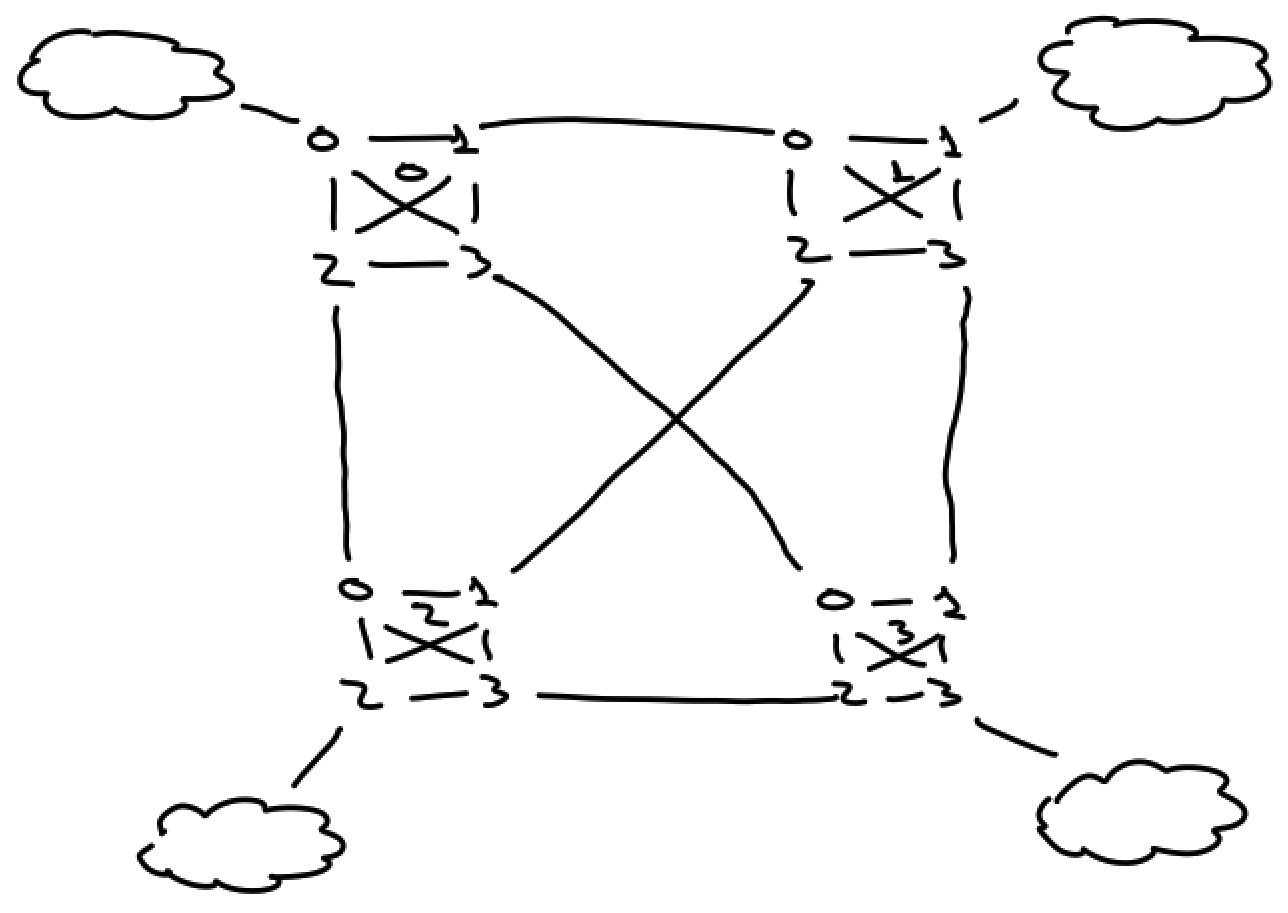
\includegraphics[width=\linewidth]{figures/no-canonica-internet.png}
        \caption{\label{fig:no-canonica-internet} Conexión a internet en la alternativa no canónica}
    \end{subfigure}
    \begin{subfigure}{0.49\textwidth}
        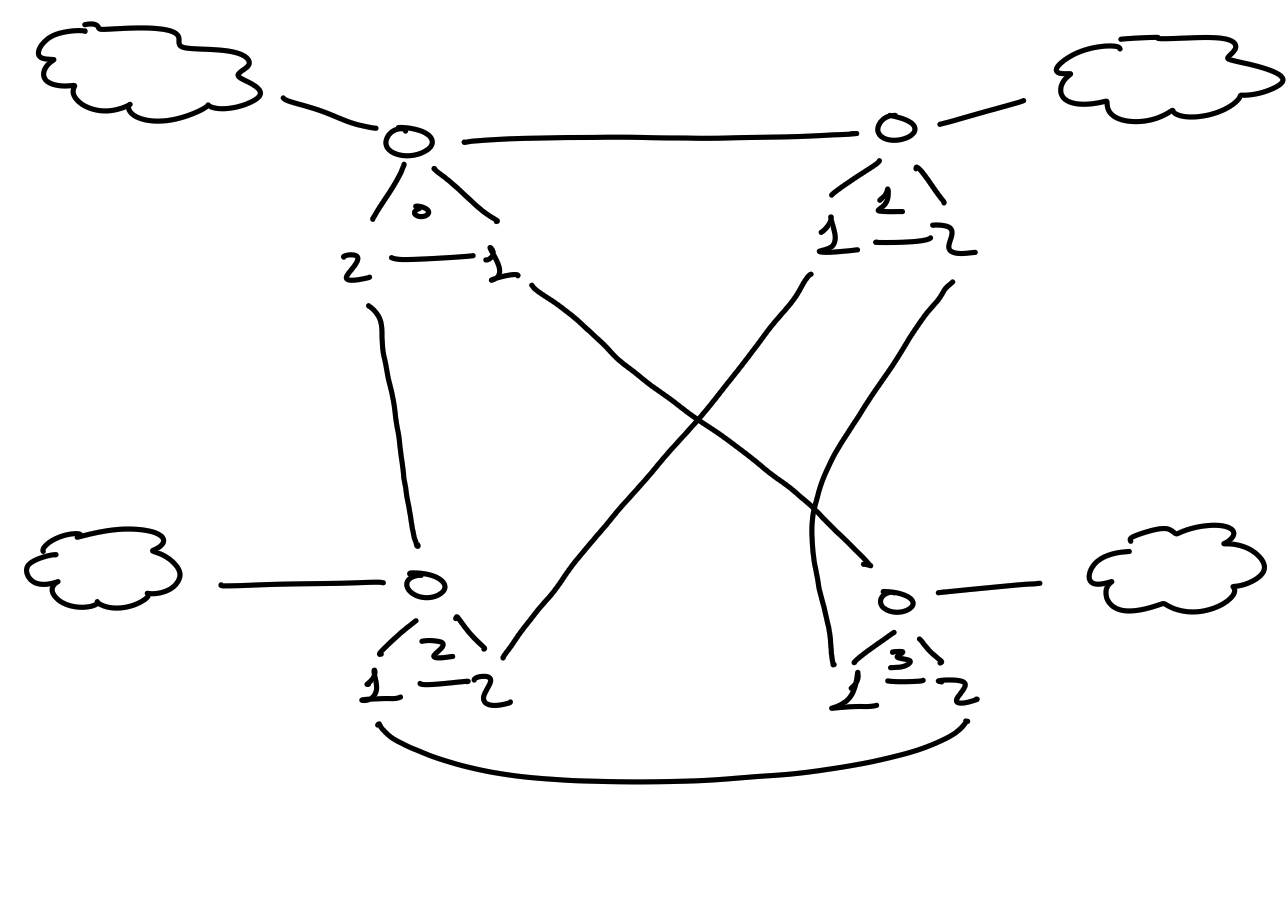
\includegraphics[width=\linewidth]{figures/canonica-internet.png}
        \caption{\label{fig:canonica-internet} Conexión a internet en la alternativa canónica}
    \end{subfigure}
    \caption{\label{fig:conexion-internet} Comparación simplificada de la conexión a internet}
\end{figure}


\chapter{Análisis de Resultados}
\label{ch:análisis-resultados}

\section{Fiabilidad}
\label{sec:fiabilidad}

La fiabilidad de la red es un aspecto crítico en cualquier sistema interconectado, ya que mide la capacidad del sistema para mantenerse operativo incluso en caso de fallos en algunos de sus componentes.

En este diseño, el objetivo de fiabilidad establecido es alcanzar un mínimo del 99.9468556\%, lo que equivale a un nivel muy alto de operatividad y resiliencia frente a fallos. Para calcular la fiabilidad de la red, se ha utilizado la fórmula de la ecuación \ref{eq:prob-fallo-enlaces}, en la cual:

\begin{itemize}
    \item $N$ es el número total de enlaces disponibles en la red
    \item $K$ es el número total de enlaces que fallan simultaneamente
    \item $p$ es la probabilidad de fallo de un enlace individual
\end{itemize}

\begin{equation} \label{eq:prob-fallo-enlaces}
    P[fallo K] = {N \choose K} \cdot p^K \cdot (1 - p)^{N - K}
\end{equation}

Para obtener un cálculo más realista, se han considerado dos escenarios: uno pesimista y otro optimista, los cuales permiten evaluar el rendimiento en situaciones con diferentes niveles de fiabilidad en los enlaces. En ambos escenarios, se ha decidido que $K$ sea igual a 6 enlaces fallidos, lo que representa aproximadamente el 5\% del total de enlaces, un margen razonable para evaluar la robustez del sistema.

\subsection{Escenario Pesimista}
\label{subsec:escenario-pesimista}

En el escenario pesimista, se considera que la probabilidad de fallo de un enlace es relativamente alta. Se ha asumido que la probabilidad de que un enlace falle es de $1 - 0.996079$, lo que indica que cada enlace tiene una pequeña pero significativa posibilidad de fallo.

Al aplicar la fórmula mencionada previamente (ecuación \ref{eq:prob-fallo-enlaces}), se obtiene una fiabilidad global de $99.99915181\%$. Este resultado demuestra que, incluso bajo condiciones pesimistas, la red supera con creces el objetivo mínimo de fiabilidad del $99.9468556\%$. 

Esto es un indicativo positivo, ya que implica que la red es capaz de mantener su funcionamiento casi perfecto incluso en circunstancias adversas, donde hasta el $5\%$ de los enlaces no funcionan.

Cabe destacar que, al cumplir el objetivo de fiabilidad en el escenario pesimista, podría parecer innecesario realizar el cálculo en el escenario optimista. Sin embargo, se llevará a cabo para tener una visión completa del desempeño del sistema bajo diferentes condiciones.

\subsection{Escenario Optimista}
\label{subsec:escenario-optimista}


En el escenario optimista, se asume que los enlaces tienen una probabilidad de fallo mucho menor. En este caso, la probabilidad de fallo de un enlace se ha establecido en $1 - 0.999850$, lo que refleja un sistema de interconexión altamente confiable, donde los fallos son extremadamente raros.

Al introducir esta probabilidad en la fórmula correspondiente (ecuación \ref{eq:prob-fallo-enlaces}), se obtiene un valor de fiabilidad global prácticamente perfecto, alcanzando un impresionante $99.999999999995909843069\%$. 

Este resultado es esencialmente un $100\%$, lo que indica que, en un escenario donde los enlaces fallan muy raramente, la red es capaz de operar sin interrupciones apreciables.

Este escenario optimista confirma que, bajo condiciones ideales, el sistema ofrece una fiabilidad excepcional, garantizando un nivel de servicio casi continuo y asegurando que el impacto de cualquier fallo sea mínimo.

\section{Análisis de Costes}
\label{sec:análisis-costes}

Una vez presentada la arquitectura de la red al completo, junto con sus necesidades de capacidad, se procede a realizar una estimación del coste total. Este coste está dividido en 2 partes: coste de la maquinaria y coste de los enlaces.

\subsection{Coste de la Maquinaria}
\label{subsec:coste-maquinaria}

Para poder realizar una estimación del coste de la maquinaria de la red, hay que hacer un recuento de todos los elementos empleados: $4545$ servidores, $240$ racks y $240$ routers. El precio resultante es:

\begin{itemize}
    \item $4545 \text{ servidores} \cdot 7000 €/\text{servidor} = 31815000 €$
    \item $240 \text{ racks} \cdot 10000 €/\text{rack} = 2400000 €$
    \item $240 \text{ routers} \cdot 6000 €/router = 1440000 €$
\end{itemize}

Total maquinaria = $35655000 €$

\subsection{Coste de los Enlaces}
\label{subsec:coste-enlaces}

Se ha supuesto un tráfico homogéneo a lo largo de toda la red, es decir, que se distribuye uniformemente entre todos los racks. Este enfoque permite simplificar los cálculos y dimensionar la infraestructura más eficientemente. En particular, el tráfico pico a cubrir es de $1.5 \cdot 10^{13}$ bps (15 Tbps). Dado que la red está compuesta por 240 racks, esto se traduce en aproximadamente 58.2 Gbps por rack.

Para asegurar que cada rack tenga capacidad suficiente para manejar este volumen de tráfico, se ha optado por utilizar enlaces de $100$ Gbps. Esta elección responde a dos razones clave:

\begin{enumerate}
    \item Capacidad adicional: Al seleccionar enlaces de 100 Gbps, se garantiza un margen por encima del tráfico homogéneo esperado, lo que proporciona flexibilidad en caso de que el tráfico en algún rack aumente temporalmente. Este enfoque previene cuellos de botella y asegura que los racks puedan manejar cargas más altas sin comprometer el rendimiento general de la red.
    \item Simplicidad en las conexiones: Aunque podría ser más económico utilizar dos enlaces de 50 Gbps en lugar de uno de 100 Gbps, la preferencia por un único enlace responde al deseo de simplificar la infraestructura de red. Al reducir el número de conexiones físicas, se disminuye la complejidad del cableado, se mejora la gestión de la red y se minimizan los puntos de fallo potenciales. Además, la utilización de un solo enlace reduce la necesidad de equilibrar tráfico entre múltiples conexiones, lo que puede complicar el diseño y la operación de la red.
\end{enumerate}

\section{Routing}
\label{sec:routing}

Lo primero que debe considerarse a la hora de diseñar el routing en una red dragonfly es que se trata de una topología que solo alcanza su máximo potencial con algoritmos de routing dinámico. 

Como se ha presentado en la elección de topolgía, una de las ventajas de este tipo de red es la tolerancia a fallos. Existe más de un camino entre dos nodos. El camino más veloz en saltos entre dos nodos de la red siempre es único y tiene exactamente tres saltos asumiendo que la red se ha configurado de forma canónica. Pero sucede a menudo que, a medida que las redes se acercan a la saturación, los caminos con menor número de saltos entre parejas de nodos, son los primeros en saturarse. Por ello mismo, la ventaja de utilizar un algoritmo de routing dinámico es que puede incrementar el throughput de la red dirigiendo el tráfico por caminos alternativos que, a pesar de ser de mayor longitud, están menos concurridos, mejorando la eficiencia de la comunicación y distribuyendo su carga. Además, un sistema de routing estático no para aprovecharía la tolerancia a fallos de la topología.

El uso de un algoritmo de routing dinámico supera el alcance del proyecto actual, que se trata simplemente de una red didáctica. Por esto mismo se va a utilizar routing estático, aunque es importante tener el anterior dato en mente para casos de implementaciones reales.

Se presentan dos maneras diferentes de encargarse del routing estático en la red dragonfly diseñada, diferenciados por el nivel de abstracción de protocolos. Puede hacerse el routing directamente en la capa ethernet mediante switches y direcciones mac (denominado red fabric) o puede subirse una capa más al nivel ip y dirigir el tráfico por routers.

\subsection{Routing a Nivel Ethernet}
\label{subsec:routing-nivel-ethernet}

La primera solución es más eficiente por la necesidad de hardware menos complejo y la reutilización de los switches que ya se encuentran en la propia red. El problema que presenta es a la hora de documentar, automatizar y comprender la distribución de la red en términos de legibilidad.

La solución que se implementa como ejemplo de este tipo de routing se puede ver en la figura \ref{fig:ethernet-routing}.

\begin{figure}
    \centering
    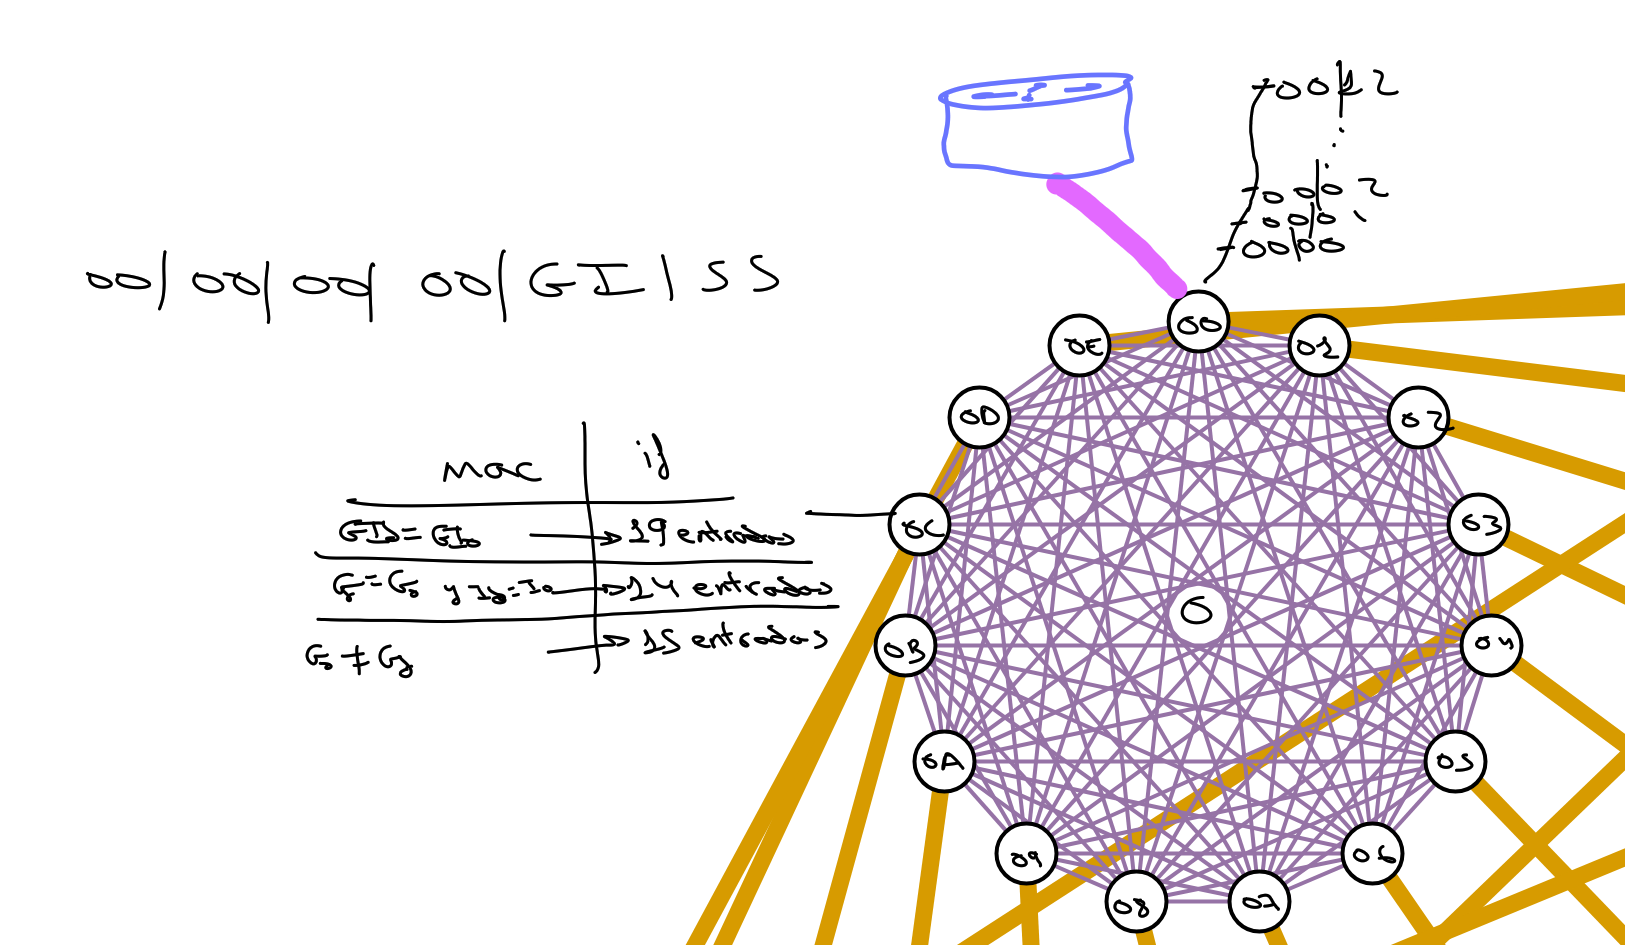
\includegraphics[width=1.0\textwidth]{figures/routing-ethernet.png}
    \caption{\label{fig:ethernet-routing} Configuración de routing a nivel ethernet}
\end{figure}

Cada rack de la red que se presentó en el diagrama anterior (figura \ref{fig:ethernet-routing}) utiliza su switch ''top of the rack'' para dirigir el tráfico entre el resto de racks del grupo y entre los diferentes grupos de la red. Para mejorar la legibilidad se propone alterar las direcciones mac como se muestra en la imagen para que el último byte represente el id del servidor dentro del rack (del 0 al 18 -> cabe dentro de 1 byte (0 a 255)), y el penúltimo byte indique el id del grupo en sus 4 primeros bits y el id del rack dentro del grupo en sus 4 siguientes.

El direccionamiento estático se compone de las siguientes reglas cada una con cierto número de entradas necesarias en la configuración del switch para su debido funcionamiento:

\begin{enumerate}
    \item $GI_d = GI_a$: (19 reglas necesarias) Si el rack destino es el mismo que el del switch actual, una regla  para cada uno de los servidores posibles.
    \item $G_d = G_a$: (14 reglas necesarias) Si el grupo destino es el del switch actual, una regla para cada uno de los racks posibles del grupo menos el actual.
    \item $G_d \neq G_a$: (15 reglas necesarias) Si el grupo destino no es el del switch actual, una regla para cada uno de los switches del grupo, si el camino hacia el grupo destino se alcanza por el switch actual, hacia fuera, si no, hacia el switch que tiene el camino correcto entre grupos.
\end{enumerate}

Siguiendo las reglas anteriores, se configura cada uno de los switches para que se encarguen del routing.

\subsection{Routing a Nivel IP}
\label{subsec:routing-nivel-ip}

Como alternativa al método anterior, define una forma de routing a nivel ip mediante la intervención de routers. Sería necesario un router en cada rack.

El concepto es similar, simplemente a una capa superior de abstracción y por tanto, más sencillo de configurar y mantener. Se puede ver con claridad en la figura \ref{fig:ip-routing}.

\begin{figure}
    \centering
    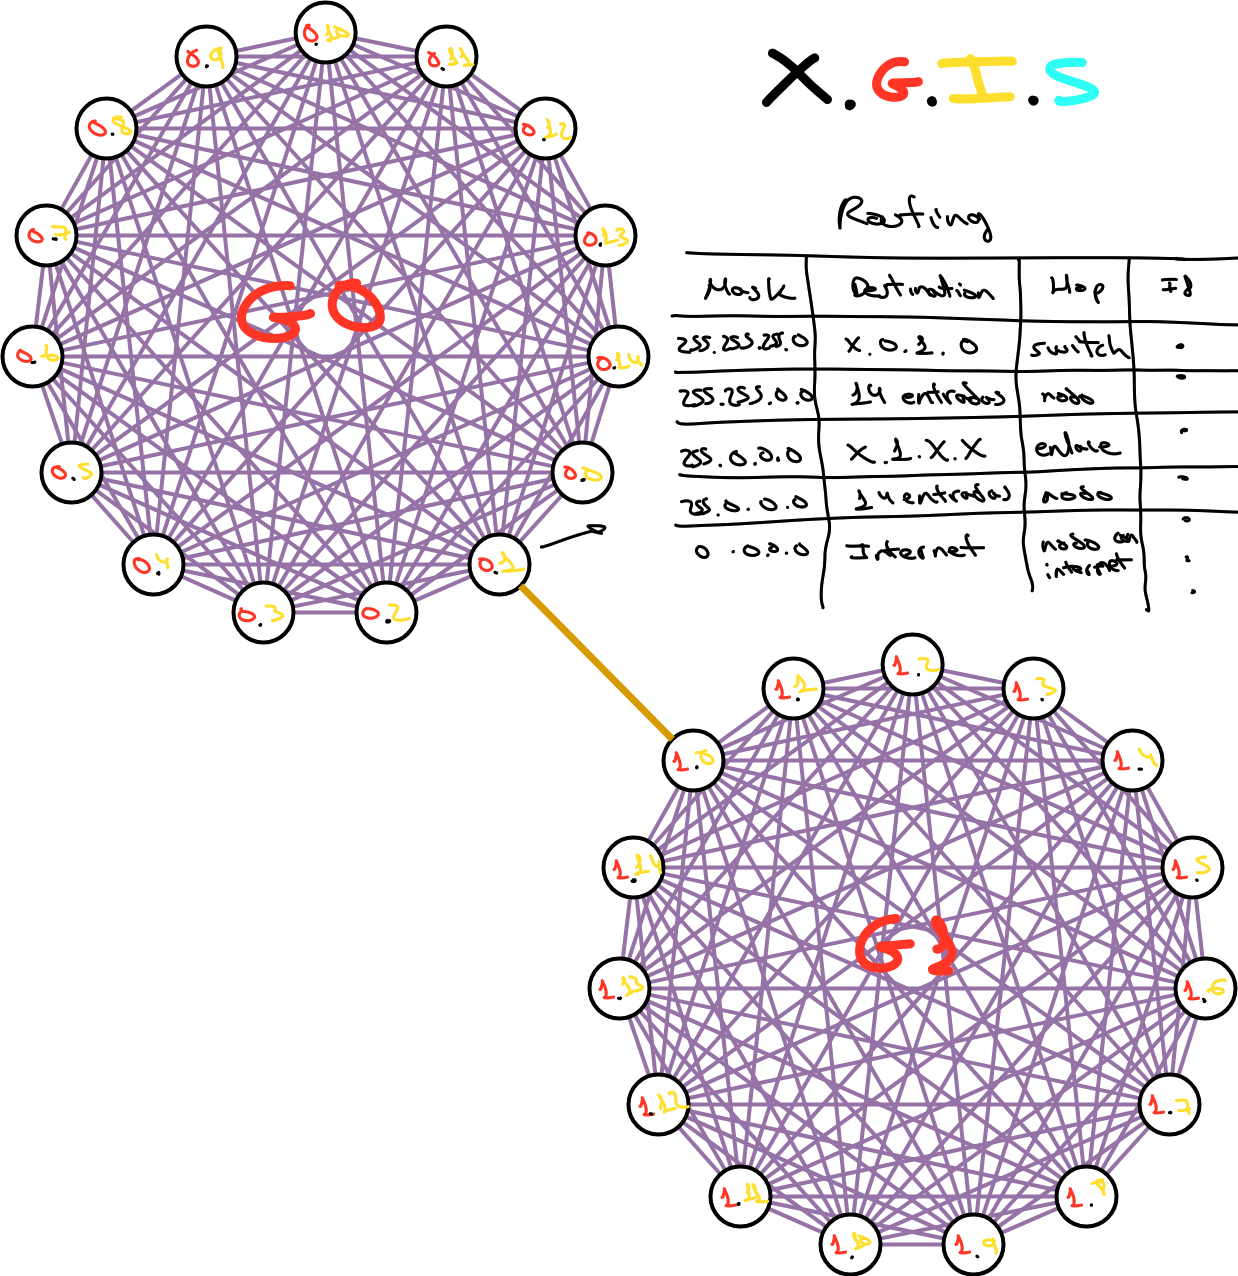
\includegraphics[width=1.0\textwidth]{figures/routing-ip.png}
    \caption{\label{fig:ip-routing} Configuración de routing a nivel ip}
\end{figure}

Como puede verse, en esta solución, las direcciones siguen un patrón similar. Se utiliza el segundo byte para representar el grupo, el tercero para el id de nodo dentro del grupo y el cuarto para el id de servidor dentro del rack. Cada dirección identifica de manera única a cada uno de los servidores de la red.

El routing en esta alternativa se basa en routing ip y sigue las mismas reglas que la solución por switches pero con direcciones ip. La manifestación de estas reglas en la tabla de direccionamiento es obviamente diferente. En la imagen puede verse el ejemplo de tabla de routing ip para el router del nodo 0.1 (grupo 0 rack 1).

\section{Firewall}

Para la seguridad de la red, se ha establecido que únicamente los nodos 0 de cada grupo (donde se ubicarán los servidores web) puedan recibir peticiones externas, siendo estos los encargados de repartir la carga de trabajo a la red. De esta manera, todos los nodos permanecen aislados exceptuando los ya mencionados. Las redes pueden enviar tráfico TCP al exterior (para transmitir los resultados de computación a quien los ha solicitado). No se permite ningún otro tipo de tráfico, ni que un ordenador externo a la red envíe tráfico a los nodos interiores.

\textbf{Política de tráfico}:
\begin{itemize}
    \item \textbf{Restricción de peticiones externas}: Se permite la recepción de tráfico desde fuera de la red únicamente a los nodos 0. No se autoriza que ningún nodo interno (nodos 1-14) reciba tráfico directo de fuentes externas.
    \item \textbf{Permiso de tráfico TCP}: Se autoriza únicamente el envío de tráfico TCP desde los nodos internos hacia el exterior (generalmente para la transmisión de resultados de operaciones). Se bloquea cualquier otro tipo de tráfico.
    \item \textbf{Aislamiento}: Se mantiene el aislamiento de los nodos del tráfico externo, exceptuando los nodos 0, estableciendo así una barrera de seguridad. Este procedimiento minimiza el riesgo de ataque, ya que se protegen completamente los nodos que realizan cálculos o tareas dentro de la red contra accesos no autorizados.
\end{itemize}

\textbf{Configuración de firewall}:
\begin{itemize}
    \item Se establece la permisión de conexiones TCP al puerto 433 de los servidores web (nodos 0) desde cualquier origen. Esto garantiza la recepción de peticiones entrantes en los nodos 0 sin restricciones, impidiendo su propagación más allá de estos.
    \item Se implementa el bloqueo de todo otro tráfico hacia los nodos 0 y dentro de la red que no esté específicamente autorizado, reforzando así la política de aislamiento.
\end{itemize}

\textbf{Otras consideraciones}:
\begin{enumerate}
   \item \textbf{Función de los nodos 0 como intermediarios}:
   \begin{itemize}
        \item \textbf{Balanceo de carga}: Al ser los únicos puntos de recepción de peticiones externas, se asigna a los nodos 0 la responsabilidad del balanceo de carga de trabajo. Este mecanismo asegura la distribución equitativa de las solicitudes de trabajo entre los nodos internos (nodos 1-14) para la optimización del rendimiento de la red.
        \item \textbf{Protección adicional mediante proxies}: Se contempla la posibilidad de que los nodos 0 funcionen como proxies o reverse proxies. Esto permite el filtrado y validación del tráfico antes de su distribución, mejorando así la seguridad y la eficiencia.
   \end{itemize}
   \item \textbf{Segmentación de la red}:
   \begin{itemize}
        \item \textbf{Segmentación lógica}: Se implementa el aislamiento de nodos como técnica de segmentación lógica dentro de la red. Esta segmentación garantiza que, en caso de compromiso de algún nodo, no se produzca la propagación del ataque a otros nodos. Se establece a los nodos 0 como único punto de contacto con el exterior, limitando así las posibilidades de ataque.
        \item \textbf{Reducción de la superficie de ataque}: Mediante la restricción del acceso a nodos internos, se logra una reducción significativa de la superficie de ataque. No es posible la explotación directa de vulnerabilidades en los nodos internos sin comprometer previamente un nodo 0.
   \end{itemize}
   \item \textbf{Uso del protocolo TCP}:
   \begin{itemize}
        \item \textbf{Justificación del tráfico TCP exclusivo}: Se selecciona TCP por ser un protocolo orientado a la conexión, garantizando la entrega de datos en orden correcto y sin pérdidas. Se prioriza este protocolo para las comunicaciones salientes al asegurar la integridad en la recepción de los resultados de los cálculos realizados por los nodos internos.
        \item \textbf{Bloqueo de otros tipos de tráfico}: Se implementa la restricción de otros tipos de tráfico, como UDP, ICMP o IP no estándar, minimizando así posibles riesgos de ataque (como DDoS mediante UDP o ICMP). Adicionalmente, se bloquean las comunicaciones no esenciales para el propósito de la red, reduciendo las oportunidades de explotación.
   \end{itemize}
\end{enumerate}

\begin{center}
\begin{array}{|c|c|c|c|c|}
    \hline
    \text{Origen} & \text{Destino} & \text{Protocolo} & \text{Puerto} & \text{Acción} \\
    \hline
    \text{ANY} & \text{10.G.0.0} & \text{TCP} & \text{433} & \text{ACCEPT} \\
    \hline
    \text{10.G.0.0} & \text{ANY} & \text{TCP} & \text{433} & \text{ACCEPT} \\
    \hline
    \text{10.G.L.0} & \text{ANY} & \text{TCP} & \text{433} & \text{ACCEPT} \\
    \hline
    \text{10.G.L.0} & \text{ANY} & \text{ANY} & \text{ANY} & \text{DROP} \\
    \hline
    \text{ANY} & \text{10.G.L.0} & \text{ANY} & \text{ANY} & \text{DROP} \\
    \hline
\end{array}
\end{center}

Donde:
\begin{itemize}
    \item G = Grupos[0-15].
    \item I = Nodos[0-14].
    \item 10.G.0.0 > Uno de los nodos del grupo esta destinado al servidor web que repartirá la
    carga de trabajo a la red.
\end{itemize}

Las peticiones solo pueden llegar a los servidores web que están en los nodos 0 de cada
grupo, desde allí la carga se repartirá en la red. Los PCs de los nodos finales solo pueden
mandar tráfico TCP a los usuarios con los cálculos que han solicitado.

\chapter{Configuración a Escala}
\label{ch:configuracion-escala}

\section{Descripción de la Nueva Topología}

Para llevar a cabo la segunda parte de la práctica, se ha decidido continuar con una topología de tipo Dragonfly, aunque, conforme a las directrices del enunciado, se ha reducido considerablemente el tamaño de dicha topología. En la figura \ref{fig:scaled-topology} se presenta el esquema de numeración de red propuesto.

\begin{figure}
    \centering
    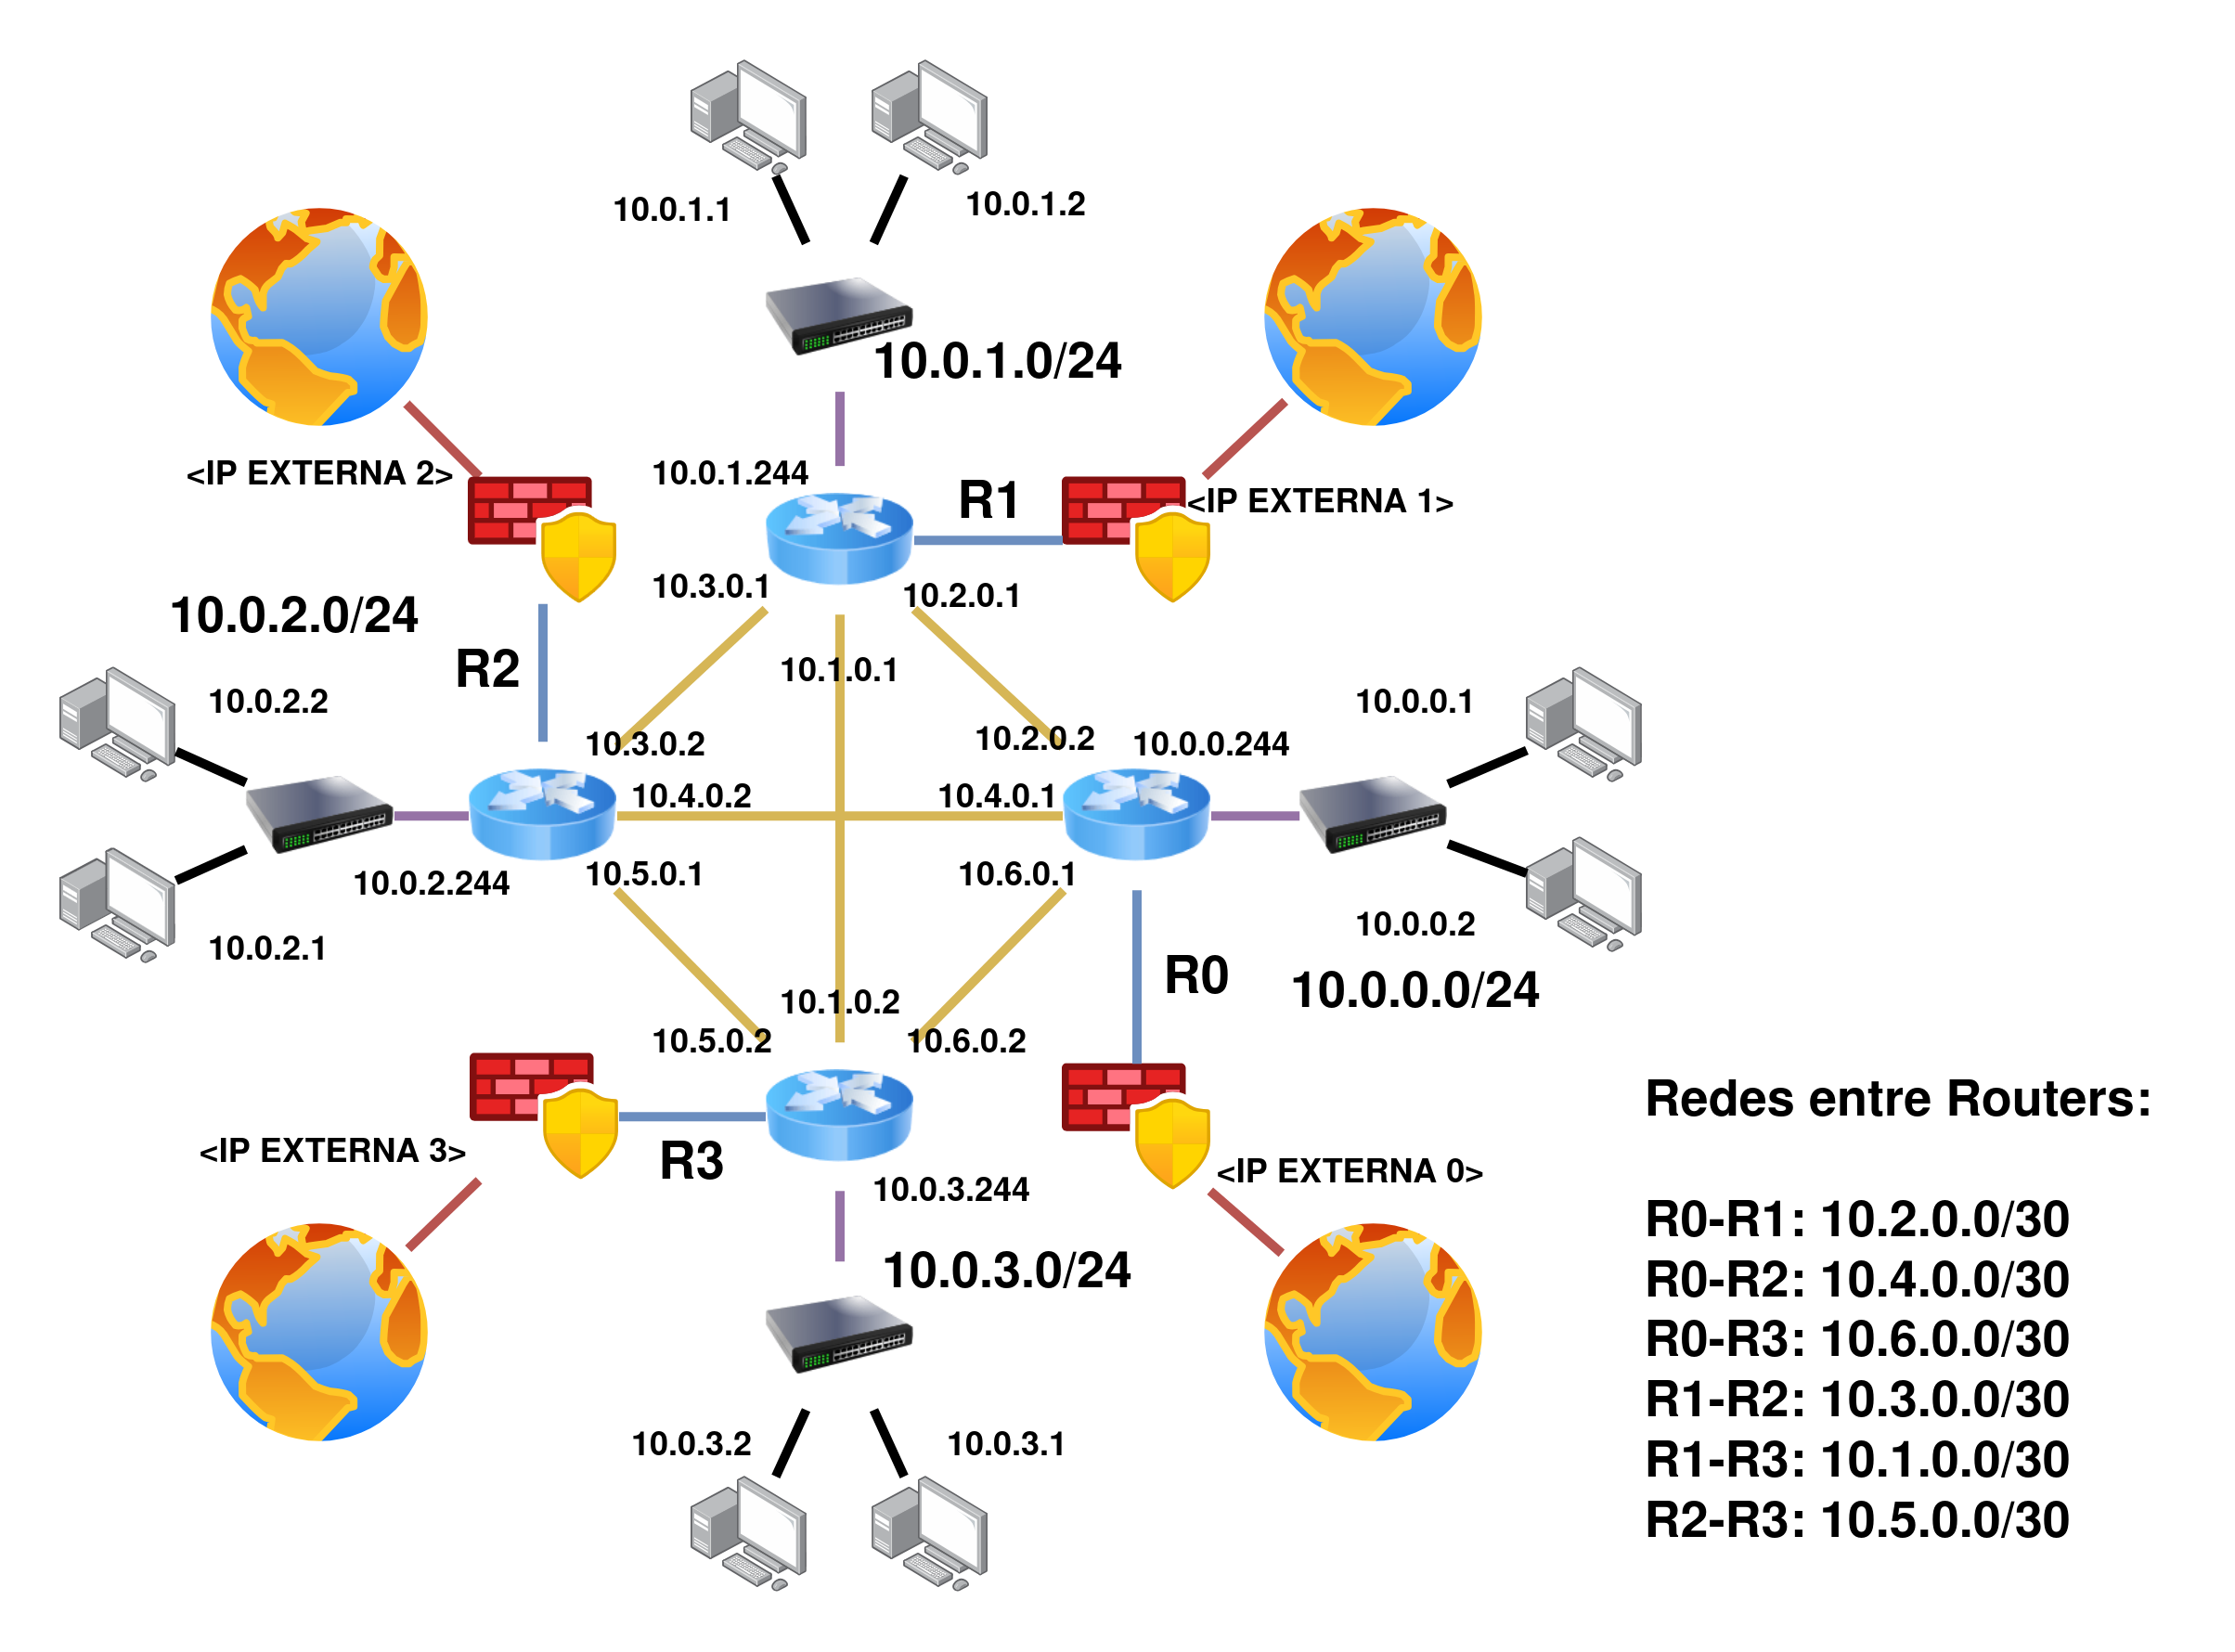
\includegraphics[width=1.0\textwidth]{figures/scaled-topology.png}
    \caption{\label{fig:scaled-topology} Topología reducida para la configuración}
\end{figure}

El nuevo esquema de numeración refleja los cambios en el número de elementos y la naturaleza de la topología empleada:
\begin{itemize}
    \item \textbf{Naturaleza:} En la primera parte se optó por una topología Dragonfly de carácter canónico. Sin embargo, para esta fase se ha configurado una Dragonfly con los parámetros: \(a = 1\), \(g = 4\), y \(h = 3\). Estos valores no cumplen con la fórmula de la Dragonfly canónica, ya que \(g = a + 1 \rightarrow 4 \neq 1 + 1\) y \(h = 1 \rightarrow 3 \neq 1\).
    \item \textbf{Número de Grupos:} Para facilitar la configuración de los routers, se han implementado 4 routers, equivalentes a 4 grupos en una topología Dragonfly.
    \item \textbf{Número de Servidores:} Por razones de gestión, el número de racks se ha reducido a 0, empleando 2 servidores en su lugar.
\end{itemize}

\section{Elementos Físicos Empleados, Configuraciones y Resultados}

\subsection{Elementos Físicos}

Para el despliegue físico de la red, se han utilizado los recursos disponibles en el laboratorio 4314. Las pruebas se realizaron empleando dos ordenadores de grupos distintos, lo cual asegura la escalabilidad de la red a partir de una comunicación exitosa entre ambos equipos. Los elementos utilizados son los siguientes:

\begin{itemize}
    \item \textbf{Servidores:} 2 ordenadores con sistema operativo Windows 11.
    \item \textbf{Routers:} 2 dispositivos SRX340.
    \item \textbf{Switches:} 2 dispositivos QFX5100.
    \item \textbf{Firewalls:} 2 dispositivos SRX340.
\end{itemize}

\subsection{Configuraciones}

\subsubsection{Servidores}

Para configurar los equipos con Windows 11, es necesario realizar varios ajustes que permitan una conexión correcta. Estas configuraciones abarcan desde la configuración de la interfaz de red hasta la adaptación del firewall de Windows para permitir el tráfico necesario.

La configuración inicial implica la asignación de la dirección IP, la máscara de subred y la puerta de enlace predeterminada. Además, en caso necesario, se puede especificar el servidor DNS, eligiendo 8.8.8.8 (DNS de Google) como preferencia. Estos pasos se muestran en la figura \ref{fig:ip-config}, y su correcta implementación se verifica en la figura \ref{fig:ip-config-check}.

\begin{figure}
    \centering
    \begin{subfigure}{0.49\textwidth}
        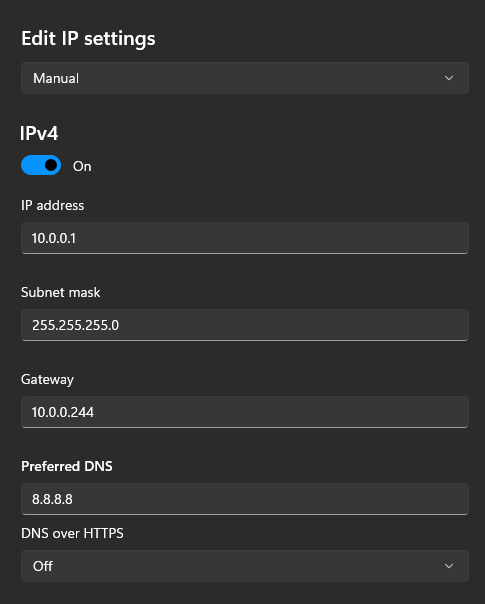
\includegraphics[width=\linewidth]{figures/ip-config-01.png}
        \caption{\label{fig:ip-config-01} Configuración de red del servidor 10.0.0.1}
    \end{subfigure}
    \begin{subfigure}{0.49\textwidth}
        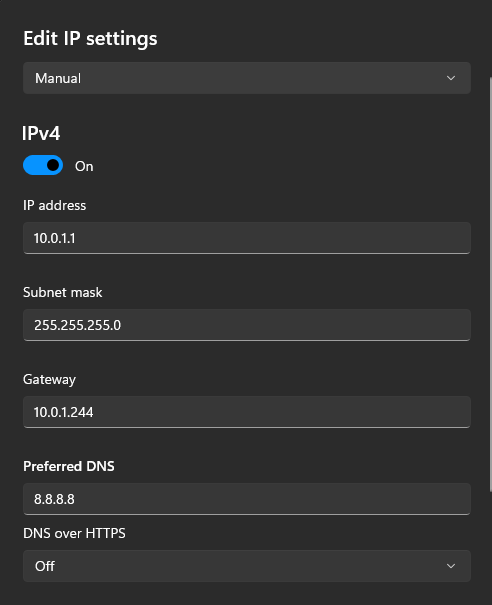
\includegraphics[width=\linewidth]{figures/ip-config-02.png}
        \caption{\label{fig:ip-config-02} Configuración de red del servidor 10.0.1.1}
    \end{subfigure}
    \caption{\label{fig:ip-config} Configuración de red de los servidores}
\end{figure}

\begin{figure}
    \centering
    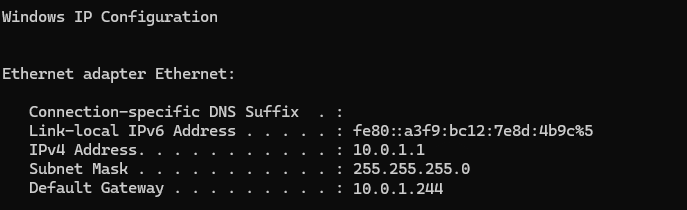
\includegraphics[width=0.9\textwidth]{figures/ip-config-check-01.png}
    \caption{\label{fig:ip-config-check} Verificación de la configuración de red del servidor 10.0.1.1}
\end{figure}

Finalmente, se debe ajustar el firewall de Windows, que por defecto bloquea la mayoría de conexiones entrantes, incluyendo el protocolo ICMP (ping). Para permitir la conectividad, existen dos opciones:
\begin{itemize}
    \item \textbf{Desactivar el Firewall (No recomendado):} Permite cualquier tipo de conectividad, incluso potencialmente maliciosa. Esta práctica es adecuada solo en entornos protegidos y sin acceso al exterior.
    \item \textbf{Implementar reglas en el Firewall (Recomendado):} Permite mantener el nivel de seguridad y se puede ajustar para permitir solo el tráfico necesario.
\end{itemize}

Dado que el entorno es controlado y sin acceso externo, se ha optado por desactivar temporalmente el firewall.

\subsubsection{Routers}

Se ha seleccionado el modelo SRX340 en modo router para permitir la conectividad. Es necesario ejecutar una serie de comandos de configuración en el dispositivo, que abarcan desde la configuración de interfaces hasta la adición de rutas estáticas. A continuación, se presenta el script de configuración para los 4 routers:

\paragraph{Router 0}

\begin{lstlisting}[breaklines]
# Router 0

cli
configure

# Borrar configuración de seguridad existente y habilitar modo router
delete security
set security forwarding-options family mpls mode packet-based
set security forwarding-options family iso mode packet-based
set security forwarding-options family inet6 mode packet-based

# Configuración básica
set system host-name R0

# Interfaces
set interfaces ge-0/0/0 unit 0 family inet address 10.0.0.244/24
set interfaces ge-0/0/1 unit 0 family inet address 10.2.0.2/30
set interfaces ge-0/0/2 unit 0 family inet address 10.4.0.1/30
set interfaces ge-0/0/3 unit 0 family inet address 10.6.0.1/30

# Rutas estáticas
set routing-options static route 10.0.1.0/24 next-hop 10.2.0.1
set routing-options static route 10.0.2.0/24 next-hop 10.4.0.2
set routing-options static route 10.0.3.0/24 next-hop 10.6.0.2
set routing-options static route 10.1.0.0/30 next-hop 10.2.0.1
set routing-options static route 10.3.0.0/30 next-hop 10.4.0.2
set routing-options static route 10.5.0.0/30 next-hop 10.6.0.2

commit
\end{lstlisting}

\paragraph{Router 1}

\begin{lstlisting}[breaklines]
# Router 1

cli
configure

# Borrar configuración de seguridad existente y habilitar modo router
delete security
set security forwarding-options family mpls mode packet-based
set security forwarding-options family iso mode packet-based
set security forwarding-options family inet6 mode packet-based

# Configuración básica
set system host-name R1

# Interfaces
set interfaces ge-0/0/0 unit 0 family inet address 10.0.1.244/24
set interfaces ge-0/0/1 unit 0 family inet address 10.2.0.1/30
set interfaces ge-0/0/2 unit 0 family inet address 10.1.0.1/30
set interfaces ge-0/0/3 unit 0 family inet address 10.3.0.1/30

# Rutas estáticas
set routing-options static route 10.0.0.0/24 next-hop 10.2.0.2
set routing-options static route 10.0.2.0/24 next-hop 10.3.0.2
set routing-options static route 10.0.3.0/24 next-hop 10.1.0.2
set routing-options static route 10.4.0.0/30 next-hop 10.2.0.2
set routing-options static route 10.5.0.0/30 next-hop 10.3.0.2
set routing-options static route 10.6.0.0/30 next-hop 10.1.0.2

commit
\end{lstlisting}

\paragraph{Router 2}

\begin{lstlisting}[breaklines]
# Router 2

cli
configure

# Borrar configuración de seguridad existente y habilitar modo router
delete security
set security forwarding-options family mpls mode packet-based
set security forwarding-options family iso mode packet-based
set security forwarding-options family inet6 mode packet-based

# Configuración básica
set system host-name R2

# Interfaces
set interfaces ge-0/0/0 unit 0 family inet address 10.0.2.244/24
set interfaces ge-0/0/1 unit 0 family inet address 10.4.0.2/30
set interfaces ge-0/0/2 unit 0 family inet address 10.3.0.2/30
set interfaces ge-0/0/3 unit 0 family inet address 10.5.0.1/30

# Rutas estáticas
set routing-options static route 10.0.0.0/24 next-hop 10.4.0.1
set routing-options static route 10.0.1.0/24 next-hop 10.3.0.1
set routing-options static route 10.0.3.0/24 next-hop 10.5.0.2
set routing-options static route 10.1.0.0/30 next-hop 10.3.0.1
set routing-options static route 10.2.0.0/30 next-hop 10.4.0.1
set routing-options static route 10.6.0.0/30 next-hop 10.5.0.2

commit   
\end{lstlisting}

\paragraph{Router 3}

\begin{lstlisting}[breaklines]
# Router 3

cli
configure

# Borrar configuración de seguridad existente y habilitar modo router
delete security
set security forwarding-options family mpls mode packet-based
set security forwarding-options family iso mode packet-based
set security forwarding-options family inet6 mode packet-based

# Configuración básica
set system host-name R3

# Interfaces
set interfaces ge-0/0/0 unit 0 family inet address 10.0.3.244/24
set interfaces ge-0/0/1 unit 0 family inet address 10.6.0.2/30
set interfaces ge-0/0/2 unit 0 family inet address 10.1.0.2/30
set interfaces ge-0/0/3 unit 0 family inet address 10.5.0.2/30

# Rutas estáticas
set routing-options static route 10.0.0.0/24 next-hop 10.6.0.1
set routing-options static route 10.0.1.0/24 next-hop 10.1.0.1
set routing-options static route 10.0.2.0/24 next-hop 10.5.0.1
set routing-options static route 10.2.0.0/30 next-hop 10.6.0.1
set routing-options static route 10.3.0.0/30 next-hop 10.5.0.1
set routing-options static route 10.4.0.0/30 next-hop 10.1.0.1

commit
\end{lstlisting}

\subsubsection{Firewalls}

Los firewalls estarán orientados hacia internet y únicamente permitirán tráfico HTTP. La configuración predeterminada en los firewalls con JUNOS es restrictiva; por ello, se deben ejecutar los siguientes comandos para permitir el tráfico HTTP:

\begin{lstlisting}[breaklines]
# Firewall

cli
configure

# Asignar interfaces a zonas
set security zones security-zone trust interfaces ge-0/0/0  # Red interna
set security zones security-zone untrust interfaces ge-0/0/1  # Internet

# Permitir servicios específicos en la interfaz interna
set security zones security-zone trust interfaces ge-0/0/0 host-inbound-traffic system-services ssh
set security zones security-zone trust interfaces ge-0/0/0 host-inbound-traffic system-services ping

# Opcional: Permitir servicios específicos en la interfaz externa
set security zones security-zone untrust interfaces ge-0/0/1 host-inbound-traffic system-services ping
set security zones security-zone untrust interfaces ge-0/0/1 host-inbound-traffic system-services ssh

commit
\end{lstlisting}

\subsubsection{Switches}

En el caso de los dispositivos QFX5100, no es necesario realizar configuraciones adicionales para lograr un funcionamiento básico. En esta modalidad, el equipo conmuta tramas Ethernet sin aplicar reglas o restricciones adicionales.

\end{document}
